%! TeX program = xelatex
\documentclass[11pt,english]{report}

%%%%%%%%%%%%%%%%%%%%%%%%%%%%%%%%%
% PACKAGE IMPORTS
%%%%%%%%%%%%%%%%%%%%%%%%%%%%%%%%%


\usepackage[tmargin=2cm,rmargin=1in,lmargin=1in,margin=0.85in,bmargin=2cm,footskip=.2in]{geometry}
\usepackage{amsmath,amsfonts,amsthm,amssymb,mathtools}
\usepackage[varbb]{newpxmath}
\usepackage{xfrac}
\usepackage[makeroom]{cancel}
\usepackage{mathtools}
\usepackage{bookmark}
\usepackage{enumitem}
\usepackage{hyperref,theoremref}
\hypersetup{
	pdftitle={Assignment},
	colorlinks=true, linkcolor=doc!90,
	bookmarksnumbered=true,
	bookmarksopen=true
}
\usepackage[most,many,breakable]{tcolorbox}
\usepackage{xcolor}
\usepackage{varwidth}
\usepackage{varwidth}
\usepackage{etoolbox}
%\usepackage{authblk}
\usepackage{nameref}
\usepackage{multicol,array}
\usepackage{tikz-cd}
\usepackage[ruled,vlined,linesnumbered]{algorithm2e}
\usepackage{comment} % enables the use of multi-line comments (\ifx \fi) 
\usepackage{import}
\usepackage{xifthen}
\usepackage{pdfpages}
\usepackage{transparent}

\newcommand\mycommfont[1]{\footnotesize\ttfamily\textcolor{blue}{#1}}
\SetCommentSty{mycommfont}
\newcommand{\incfig}[1]{%
    \def\svgwidth{\columnwidth}
    \import{./figures/}{#1.pdf_tex}
}

\usepackage{tikzsymbols}
\renewcommand\qedsymbol{$\Laughey$}


%\usepackage{import}
%\usepackage{xifthen}
%\usepackage{pdfpages}
%\usepackage{transparent}


%%%%%%%%%%%%%%%%%%%%%%%%%%%%%%
% SELF MADE COLORS
%%%%%%%%%%%%%%%%%%%%%%%%%%%%%%



\definecolor{myg}{RGB}{56, 140, 70}
\definecolor{myb}{RGB}{45, 111, 177}
\definecolor{myr}{RGB}{199, 68, 64}
\definecolor{mytheorembg}{HTML}{F2F2F9}
\definecolor{mytheoremfr}{HTML}{00007B}
\definecolor{mylenmabg}{HTML}{FFFAF8}
\definecolor{mylenmafr}{HTML}{983b0f}
\definecolor{mypropbg}{HTML}{f2fbfc}
\definecolor{mypropfr}{HTML}{191971}
\definecolor{myexamplebg}{HTML}{F2FBF8}
\definecolor{myexamplefr}{HTML}{88D6D1}
\definecolor{myexampleti}{HTML}{2A7F7F}
\definecolor{mydefinitbg}{HTML}{E5E5FF}
\definecolor{mydefinitfr}{HTML}{3F3FA3}
\definecolor{notesgreen}{RGB}{0,162,0}
\definecolor{myp}{RGB}{197, 92, 212}
\definecolor{mygr}{HTML}{2C3338}
\definecolor{myred}{RGB}{127,0,0}
\definecolor{myyellow}{RGB}{169,121,69}
\definecolor{myexercisebg}{HTML}{F2FBF8}
\definecolor{myexercisefg}{HTML}{88D6D1}


%%%%%%%%%%%%%%%%%%%%%%%%%%%%
% TCOLORBOX SETUPS
%%%%%%%%%%%%%%%%%%%%%%%%%%%%

\setlength{\parindent}{1cm}
%================================
% THEOREM BOX
%================================

\tcbuselibrary{theorems,skins,hooks}
\newtcbtheorem[number within=section]{Theorem}{Theorem}
{%
	enhanced,
	breakable,
	colback = mytheorembg,
	frame hidden,
	boxrule = 0sp,
	borderline west = {2pt}{0pt}{mytheoremfr},
	sharp corners,
	detach title,
	before upper = \tcbtitle\par\smallskip,
	coltitle = mytheoremfr,
	fonttitle = \bfseries\sffamily,
	description font = \mdseries,
	separator sign none,
	segmentation style={solid, mytheoremfr},
}
{th}

\tcbuselibrary{theorems,skins,hooks}
\newtcbtheorem[number within=chapter]{theorem}{Theorem}
{%
	enhanced,
	breakable,
	colback = mytheorembg,
	frame hidden,
	boxrule = 0sp,
	borderline west = {2pt}{0pt}{mytheoremfr},
	sharp corners,
	detach title,
	before upper = \tcbtitle\par\smallskip,
	coltitle = mytheoremfr,
	fonttitle = \bfseries\sffamily,
	description font = \mdseries,
	separator sign none,
	segmentation style={solid, mytheoremfr},
}
{th}


\tcbuselibrary{theorems,skins,hooks}
\newtcolorbox{Theoremcon}
{%
	enhanced
	,breakable
	,colback = mytheorembg
	,frame hidden
	,boxrule = 0sp
	,borderline west = {2pt}{0pt}{mytheoremfr}
	,sharp corners
	,description font = \mdseries
	,separator sign none
}

%================================
% Corollery
%================================
\tcbuselibrary{theorems,skins,hooks}
\newtcbtheorem[number within=section]{Corollary}{Corollary}
{%
	enhanced
	,breakable
	,colback = myp!10
	,frame hidden
	,boxrule = 0sp
	,borderline west = {2pt}{0pt}{myp!85!black}
	,sharp corners
	,detach title
	,before upper = \tcbtitle\par\smallskip
	,coltitle = myp!85!black
	,fonttitle = \bfseries\sffamily
	,description font = \mdseries
	,separator sign none
	,segmentation style={solid, myp!85!black}
}
{th}
\tcbuselibrary{theorems,skins,hooks}
\newtcbtheorem[number within=chapter]{corollary}{Corollary}
{%
	enhanced
	,breakable
	,colback = myp!10
	,frame hidden
	,boxrule = 0sp
	,borderline west = {2pt}{0pt}{myp!85!black}
	,sharp corners
	,detach title
	,before upper = \tcbtitle\par\smallskip
	,coltitle = myp!85!black
	,fonttitle = \bfseries\sffamily
	,description font = \mdseries
	,separator sign none
	,segmentation style={solid, myp!85!black}
}
{th}


%================================
% LENMA
%================================

\tcbuselibrary{theorems,skins,hooks}
\newtcbtheorem[number within=section]{Lenma}{Lenma}
{%
	enhanced,
	breakable,
	colback = mylenmabg,
	frame hidden,
	boxrule = 0sp,
	borderline west = {2pt}{0pt}{mylenmafr},
	sharp corners,
	detach title,
	before upper = \tcbtitle\par\smallskip,
	coltitle = mylenmafr,
	fonttitle = \bfseries\sffamily,
	description font = \mdseries,
	separator sign none,
	segmentation style={solid, mylenmafr},
}
{th}

\tcbuselibrary{theorems,skins,hooks}
\newtcbtheorem[number within=chapter]{lenma}{Lenma}
{%
	enhanced,
	breakable,
	colback = mylenmabg,
	frame hidden,
	boxrule = 0sp,
	borderline west = {2pt}{0pt}{mylenmafr},
	sharp corners,
	detach title,
	before upper = \tcbtitle\par\smallskip,
	coltitle = mylenmafr,
	fonttitle = \bfseries\sffamily,
	description font = \mdseries,
	separator sign none,
	segmentation style={solid, mylenmafr},
}
{th}


%================================
% PROPOSITION
%================================

\tcbuselibrary{theorems,skins,hooks}
\newtcbtheorem[number within=section]{Prop}{Proposition}
{%
	enhanced,
	breakable,
	colback = mypropbg,
	frame hidden,
	boxrule = 0sp,
	borderline west = {2pt}{0pt}{mypropfr},
	sharp corners,
	detach title,
	before upper = \tcbtitle\par\smallskip,
	coltitle = mypropfr,
	fonttitle = \bfseries\sffamily,
	description font = \mdseries,
	separator sign none,
	segmentation style={solid, mypropfr},
}
{th}

\tcbuselibrary{theorems,skins,hooks}
\newtcbtheorem[number within=chapter]{prop}{Proposition}
{%
	enhanced,
	breakable,
	colback = mypropbg,
	frame hidden,
	boxrule = 0sp,
	borderline west = {2pt}{0pt}{mypropfr},
	sharp corners,
	detach title,
	before upper = \tcbtitle\par\smallskip,
	coltitle = mypropfr,
	fonttitle = \bfseries\sffamily,
	description font = \mdseries,
	separator sign none,
	segmentation style={solid, mypropfr},
}
{th}


%================================
% CLAIM
%================================

\tcbuselibrary{theorems,skins,hooks}
\newtcbtheorem[number within=section]{claim}{Claim}
{%
	enhanced
	,breakable
	,colback = myg!10
	,frame hidden
	,boxrule = 0sp
	,borderline west = {2pt}{0pt}{myg}
	,sharp corners
	,detach title
	,before upper = \tcbtitle\par\smallskip
	,coltitle = myg!85!black
	,fonttitle = \bfseries\sffamily
	,description font = \mdseries
	,separator sign none
	,segmentation style={solid, myg!85!black}
}
{th}



%================================
% Exercise
%================================

\tcbuselibrary{theorems,skins,hooks}
\newtcbtheorem[number within=section]{Exercise}{Exercise}
{%
	enhanced,
	breakable,
	colback = myexercisebg,
	frame hidden,
	boxrule = 0sp,
	borderline west = {2pt}{0pt}{myexercisefg},
	sharp corners,
	detach title,
	before upper = \tcbtitle\par\smallskip,
	coltitle = myexercisefg,
	fonttitle = \bfseries\sffamily,
	description font = \mdseries,
	separator sign none,
	segmentation style={solid, myexercisefg},
}
{th}

\tcbuselibrary{theorems,skins,hooks}
\newtcbtheorem[number within=chapter]{exercise}{Exercise}
{%
	enhanced,
	breakable,
	colback = myexercisebg,
	frame hidden,
	boxrule = 0sp,
	borderline west = {2pt}{0pt}{myexercisefg},
	sharp corners,
	detach title,
	before upper = \tcbtitle\par\smallskip,
	coltitle = myexercisefg,
	fonttitle = \bfseries\sffamily,
	description font = \mdseries,
	separator sign none,
	segmentation style={solid, myexercisefg},
}
{th}

%================================
% EXAMPLE BOX
%================================

\newtcbtheorem[number within=section]{Example}{Example}
{%
	colback = myexamplebg
	,breakable
	,colframe = myexamplefr
	,coltitle = myexampleti
	,boxrule = 1pt
	,sharp corners
	,detach title
	,before upper=\tcbtitle\par\smallskip
	,fonttitle = \bfseries
	,description font = \mdseries
	,separator sign none
	,description delimiters parenthesis
}
{ex}

\newtcbtheorem[number within=chapter]{example}{Example}
{%
	colback = myexamplebg
	,breakable
	,colframe = myexamplefr
	,coltitle = myexampleti
	,boxrule = 1pt
	,sharp corners
	,detach title
	,before upper=\tcbtitle\par\smallskip
	,fonttitle = \bfseries
	,description font = \mdseries
	,separator sign none
	,description delimiters parenthesis
}
{ex}

%================================
% DEFINITION BOX
%================================

\newtcbtheorem[number within=section]{Definition}{Definition}{enhanced,
	before skip=2mm,after skip=2mm, colback=red!5,colframe=red!80!black,boxrule=0.5mm,
	attach boxed title to top left={xshift=1cm,yshift*=1mm-\tcboxedtitleheight}, varwidth boxed title*=-3cm,
	boxed title style={frame code={
					\path[fill=tcbcolback]
					([yshift=-1mm,xshift=-1mm]frame.north west)
					arc[start angle=0,end angle=180,radius=1mm]
					([yshift=-1mm,xshift=1mm]frame.north east)
					arc[start angle=180,end angle=0,radius=1mm];
					\path[left color=tcbcolback!60!black,right color=tcbcolback!60!black,
						middle color=tcbcolback!80!black]
					([xshift=-2mm]frame.north west) -- ([xshift=2mm]frame.north east)
					[rounded corners=1mm]-- ([xshift=1mm,yshift=-1mm]frame.north east)
					-- (frame.south east) -- (frame.south west)
					-- ([xshift=-1mm,yshift=-1mm]frame.north west)
					[sharp corners]-- cycle;
				},interior engine=empty,
		},
	fonttitle=\bfseries,
	title={#2},#1}{def}
\newtcbtheorem[number within=chapter]{definition}{Definition}{enhanced,
	before skip=2mm,after skip=2mm, colback=red!5,colframe=red!80!black,boxrule=0.5mm,
	attach boxed title to top left={xshift=1cm,yshift*=1mm-\tcboxedtitleheight}, varwidth boxed title*=-3cm,
	boxed title style={frame code={
					\path[fill=tcbcolback]
					([yshift=-1mm,xshift=-1mm]frame.north west)
					arc[start angle=0,end angle=180,radius=1mm]
					([yshift=-1mm,xshift=1mm]frame.north east)
					arc[start angle=180,end angle=0,radius=1mm];
					\path[left color=tcbcolback!60!black,right color=tcbcolback!60!black,
						middle color=tcbcolback!80!black]
					([xshift=-2mm]frame.north west) -- ([xshift=2mm]frame.north east)
					[rounded corners=1mm]-- ([xshift=1mm,yshift=-1mm]frame.north east)
					-- (frame.south east) -- (frame.south west)
					-- ([xshift=-1mm,yshift=-1mm]frame.north west)
					[sharp corners]-- cycle;
				},interior engine=empty,
		},
	fonttitle=\bfseries,
	title={#2},#1}{def}



%================================
% Solution BOX
%================================

\makeatletter
\newtcbtheorem{question}{Question}{enhanced,
	breakable,
	colback=white,
	colframe=myb!80!black,
	attach boxed title to top left={yshift*=-\tcboxedtitleheight},
	fonttitle=\bfseries,
	title={#2},
	boxed title size=title,
	boxed title style={%
			sharp corners,
			rounded corners=northwest,
			colback=tcbcolframe,
			boxrule=0pt,
		},
	underlay boxed title={%
			\path[fill=tcbcolframe] (title.south west)--(title.south east)
			to[out=0, in=180] ([xshift=5mm]title.east)--
			(title.center-|frame.east)
			[rounded corners=\kvtcb@arc] |-
			(frame.north) -| cycle;
		},
	#1
}{def}
\makeatother

%================================
% SOLUTION BOX
%================================

\makeatletter
\newtcolorbox{solution}{enhanced,
	breakable,
	colback=white,
	colframe=myg!80!black,
	attach boxed title to top left={yshift*=-\tcboxedtitleheight},
	title=Solution,
	boxed title size=title,
	boxed title style={%
			sharp corners,
			rounded corners=northwest,
			colback=tcbcolframe,
			boxrule=0pt,
		},
	underlay boxed title={%
			\path[fill=tcbcolframe] (title.south west)--(title.south east)
			to[out=0, in=180] ([xshift=5mm]title.east)--
			(title.center-|frame.east)
			[rounded corners=\kvtcb@arc] |-
			(frame.north) -| cycle;
		},
}
\makeatother

%================================
% Question BOX
%================================

\makeatletter
\newtcbtheorem{qstion}{Question}{enhanced,
	breakable,
	colback=white,
	colframe=mygr,
	attach boxed title to top left={yshift*=-\tcboxedtitleheight},
	fonttitle=\bfseries,
	title={#2},
	boxed title size=title,
	boxed title style={%
			sharp corners,
			rounded corners=northwest,
			colback=tcbcolframe,
			boxrule=0pt,
		},
	underlay boxed title={%
			\path[fill=tcbcolframe] (title.south west)--(title.south east)
			to[out=0, in=180] ([xshift=5mm]title.east)--
			(title.center-|frame.east)
			[rounded corners=\kvtcb@arc] |-
			(frame.north) -| cycle;
		},
	#1
}{def}
\makeatother

\newtcbtheorem[number within=chapter]{wconc}{Wrong Concept}{
	breakable,
	enhanced,
	colback=white,
	colframe=myr,
	arc=0pt,
	outer arc=0pt,
	fonttitle=\bfseries\sffamily\large,
	colbacktitle=myr,
	attach boxed title to top left={},
	boxed title style={
			enhanced,
			skin=enhancedfirst jigsaw,
			arc=3pt,
			bottom=0pt,
			interior style={fill=myr}
		},
	#1
}{def}



%================================
% NOTE BOX
%================================

\usetikzlibrary{arrows,calc,shadows.blur}
\tcbuselibrary{skins}
\newtcolorbox{note}[1][]{%
	enhanced jigsaw,
	colback=gray!20!white,%
	colframe=gray!80!black,
	size=small,
	boxrule=1pt,
	title=\textbf{Note:-},
	halign title=flush center,
	coltitle=black,
	breakable,
	drop shadow=black!50!white,
	attach boxed title to top left={xshift=1cm,yshift=-\tcboxedtitleheight/2,yshifttext=-\tcboxedtitleheight/2},
	minipage boxed title=1.5cm,
	boxed title style={%
			colback=white,
			size=fbox,
			boxrule=1pt,
			boxsep=2pt,
			underlay={%
					\coordinate (dotA) at ($(interior.west) + (-0.5pt,0)$);
					\coordinate (dotB) at ($(interior.east) + (0.5pt,0)$);
					\begin{scope}
						\clip (interior.north west) rectangle ([xshift=3ex]interior.east);
						\filldraw [white, blur shadow={shadow opacity=60, shadow yshift=-.75ex}, rounded corners=2pt] (interior.north west) rectangle (interior.south east);
					\end{scope}
					\begin{scope}[gray!80!black]
						\fill (dotA) circle (2pt);
						\fill (dotB) circle (2pt);
					\end{scope}
				},
		},
	#1,
}

%%%%%%%%%%%%%%%%%%%%%%%%%%%%%%
% SELF MADE COMMANDS
%%%%%%%%%%%%%%%%%%%%%%%%%%%%%%


\newcommand{\thm}[2]{\begin{Theorem}{#1}{}#2\end{Theorem}}
\newcommand{\cor}[2]{\begin{Corollary}{#1}{}#2\end{Corollary}}
\newcommand{\mlenma}[2]{\begin{Lenma}{#1}{}#2\end{Lenma}}
\newcommand{\mprop}[2]{\begin{Prop}{#1}{}#2\end{Prop}}
\newcommand{\clm}[3]{\begin{claim}{#1}{#2}#3\end{claim}}
\newcommand{\wc}[2]{\begin{wconc}{#1}{}\setlength{\parindent}{1cm}#2\end{wconc}}
\newcommand{\thmcon}[1]{\begin{Theoremcon}{#1}\end{Theoremcon}}
\newcommand{\ex}[2]{\begin{Example}{#1}{}#2\end{Example}}
\newcommand{\dfn}[2]{\begin{Definition}[colbacktitle=red!75!black]{#1}{}#2\end{Definition}}
\newcommand{\dfnc}[2]{\begin{definition}[colbacktitle=red!75!black]{#1}{}#2\end{definition}}
\newcommand{\qs}[2]{\begin{question}{#1}{}#2\end{question}}
\newcommand{\pf}[2]{\begin{myproof}[#1]#2\end{myproof}}
\newcommand{\nt}[1]{\begin{note}#1\end{note}}

\newcommand*\circled[1]{\tikz[baseline=(char.base)]{
		\node[shape=circle,draw,inner sep=1pt] (char) {#1};}}
\newcommand\getcurrentref[1]{%
	\ifnumequal{\value{#1}}{0}
	{??}
	{\the\value{#1}}%
}
\newcommand{\getCurrentSectionNumber}{\getcurrentref{section}}
\newenvironment{myproof}[1][\proofname]{%
	\proof[\bfseries #1: ]%
}{\endproof}

\newcommand{\mclm}[2]{\begin{myclaim}[#1]#2\end{myclaim}}
\newenvironment{myclaim}[1][\claimname]{\proof[\bfseries #1: ]}{}

\newcounter{mylabelcounter}

\makeatletter
\newcommand{\setword}[2]{%
	\phantomsection
	#1\def\@currentlabel{\unexpanded{#1}}\label{#2}%
}
\makeatother




\tikzset{
	symbol/.style={
			draw=none,
			every to/.append style={
					edge node={node [sloped, allow upside down, auto=false]{$#1$}}}
		}
}


% deliminators
\DeclarePairedDelimiter{\abs}{\lvert}{\rvert}
\DeclarePairedDelimiter{\norm}{\lVert}{\rVert}

\DeclarePairedDelimiter{\ceil}{\lceil}{\rceil}
\DeclarePairedDelimiter{\floor}{\lfloor}{\rfloor}
\DeclarePairedDelimiter{\round}{\lfloor}{\rceil}

\newsavebox\diffdbox
\newcommand{\slantedromand}{{\mathpalette\makesl{d}}}
\newcommand{\makesl}[2]{%
\begingroup
\sbox{\diffdbox}{$\mathsurround=0pt#1\mathrm{#2}$}%
\pdfsave
\pdfsetmatrix{1 0 0.2 1}%
\rlap{\usebox{\diffdbox}}%
\pdfrestore
\hskip\wd\diffdbox
\endgroup
}
\newcommand{\dd}[1][]{\ensuremath{\mathop{}\!\ifstrempty{#1}{%
\slantedromand\@ifnextchar^{\hspace{0.2ex}}{\hspace{0.1ex}}}%
{\slantedromand\hspace{0.2ex}^{#1}}}}
\ProvideDocumentCommand\dv{o m g}{%
  \ensuremath{%
    \IfValueTF{#3}{%
      \IfNoValueTF{#1}{%
        \frac{\dd #2}{\dd #3}%
      }{%
        \frac{\dd^{#1} #2}{\dd #3^{#1}}%
      }%
    }{%
      \IfNoValueTF{#1}{%
        \frac{\dd}{\dd #2}%
      }{%
        \frac{\dd^{#1}}{\dd #2^{#1}}%
      }%
    }%
  }%
}
\providecommand*{\pdv}[3][]{\frac{\partial^{#1}#2}{\partial#3^{#1}}}
%  - others
\DeclareMathOperator{\Lap}{\mathcal{L}}
\DeclareMathOperator{\Var}{Var} % varience
\DeclareMathOperator{\Cov}{Cov} % covarience
\DeclareMathOperator{\E}{E} % expected

% Since the amsthm package isn't loaded

% I prefer the slanted \leq
\let\oldleq\leq % save them in case they're every wanted
\let\oldgeq\geq
\renewcommand{\leq}{\leqslant}
\renewcommand{\geq}{\geqslant}

% % redefine matrix env to allow for alignment, use r as default
% \renewcommand*\env@matrix[1][r]{\hskip -\arraycolsep
%     \let\@ifnextchar\new@ifnextchar
%     \array{*\c@MaxMatrixCols #1}}


%\usepackage{framed}
%\usepackage{titletoc}
%\usepackage{etoolbox}
%\usepackage{lmodern}


%\patchcmd{\tableofcontents}{\contentsname}{\sffamily\contentsname}{}{}

%\renewenvironment{leftbar}
%{\def\FrameCommand{\hspace{6em}%
%		{\color{myyellow}\vrule width 2pt depth 6pt}\hspace{1em}}%
%	\MakeFramed{\parshape 1 0cm \dimexpr\textwidth-6em\relax\FrameRestore}\vskip2pt%
%}
%{\endMakeFramed}

%\titlecontents{chapter}
%[0em]{\vspace*{2\baselineskip}}
%{\parbox{4.5em}{%
%		\hfill\Huge\sffamily\bfseries\color{myred}\thecontentspage}%
%	\vspace*{-2.3\baselineskip}\leftbar\textsc{\small\chaptername~\thecontentslabel}\\\sffamily}
%{}{\endleftbar}
%\titlecontents{section}
%[8.4em]
%{\sffamily\contentslabel{3em}}{}{}
%{\hspace{0.5em}\nobreak\itshape\color{myred}\contentspage}
%\titlecontents{subsection}
%[8.4em]
%{\sffamily\contentslabel{3em}}{}{}  
%{\hspace{0.5em}\nobreak\itshape\color{myred}\contentspage}



%%%%%%%%%%%%%%%%%%%%%%%%%%%%%%%%%%%%%%%%%%%
% TABLE OF CONTENTS
%%%%%%%%%%%%%%%%%%%%%%%%%%%%%%%%%%%%%%%%%%%

\usepackage{tikz}
\definecolor{doc}{RGB}{0,60,110}
\usepackage{titletoc}
\contentsmargin{0cm}
\titlecontents{chapter}[3.7pc]
{\addvspace{30pt}%
	\begin{tikzpicture}[remember picture, overlay]%
		\draw[fill=doc!60,draw=doc!60] (-7,-.1) rectangle (-0.9,.5);%
		\pgftext[left,x=-3.5cm,y=0.2cm]{\color{white}\Large\sc\bfseries Chapter\ \thecontentslabel};%
	\end{tikzpicture}\color{doc!60}\large\sc\bfseries}%
{}
{}
{\;\titlerule\;\large\sc\bfseries Page \thecontentspage
	\begin{tikzpicture}[remember picture, overlay]
		\draw[fill=doc!60,draw=doc!60] (2pt,0) rectangle (4,0.1pt);
	\end{tikzpicture}}%
\titlecontents{section}[3.7pc]
{\addvspace{2pt}}
{\contentslabel[\thecontentslabel]{2pc}}
{}
{\hfill\small \thecontentspage}
[]
\titlecontents*{subsection}[3.7pc]
{\addvspace{-1pt}\small}
{}
{}
{\ --- \small\thecontentspage}
[ \textbullet\ ][]

\makeatletter
\renewcommand{\tableofcontents}{%
	\chapter*{%
	  \vspace*{-20\p@}%
	  \begin{tikzpicture}[remember picture, overlay]%
		  \pgftext[right,x=15cm,y=0.2cm]{\color{doc!60}\Huge\sc\bfseries \contentsname};%
		  \draw[fill=doc!60,draw=doc!60] (13,-.75) rectangle (20,1);%
		  \clip (13,-.75) rectangle (20,1);
		  \pgftext[right,x=15cm,y=0.2cm]{\color{white}\Huge\sc\bfseries \contentsname};%
	  \end{tikzpicture}}%
	\@starttoc{toc}}
\makeatother


%%%%%%%%%%%%%%%%%%%%%%%%%%%%%%%%%%%%%%%%%%%
% SELF ADD PACAGES
%%%%%%%%%%%%%%%%%%%%%%%%%%%%%%%%%%%%%%%%%%%
\usepackage{xeCJK}
    \setCJKmainfont[AutoFakeBold=10]{BiauKaiTC}
    \XeTeXlinebreaklocale "zh"
    % \XeTeXlinebreakskip = 0pt plus 1pt

\usepackage{tabularx,ragged2e}
\newcolumntype{C}{>{\Centering\arraybackslash}X}
\usepackage{indentfirst}
\usepackage{longtable}
\usepackage{threeparttable}
\usepackage{float}
\usepackage{changepage}
\usepackage[title,titletoc,toc]{appendix}
\usepackage{setspace} \doublespacing

%From M275 "Topology" at SJSU
\newcommand{\id}{\mathrm{id}}
\newcommand{\taking}[1]{\xrightarrow{#1}}
\newcommand{\inv}{^{-1}}

%From M170 "Introduction to Graph Theory" at SJSU
\DeclareMathOperator{\diam}{diam}
\DeclareMathOperator{\ord}{ord}
\newcommand{\defeq}{\overset{\mathrm{def}}{=}}

%From the USAMO .tex files
\newcommand{\ts}{\textsuperscript}
\newcommand{\dg}{^\circ}
\newcommand{\ii}{\item}

% % From Math 55 and Math 145 at Harvard
% \newenvironment{subproof}[1][Proof]{%
% \begin{proof}[#1] \renewcommand{\qedsymbol}{$\blacksquare$}}%
% {\end{proof}}

\newcommand{\liff}{\leftrightarrow}
\newcommand{\lthen}{\rightarrow}
\newcommand{\opname}{\operatorname}
\newcommand{\surjto}{\twoheadrightarrow}
\newcommand{\injto}{\hookrightarrow}
\newcommand{\On}{\mathrm{On}} % ordinals
\DeclareMathOperator{\img}{im} % Image
\DeclareMathOperator{\Img}{Im} % Image
\DeclareMathOperator{\coker}{coker} % Cokernel
\DeclareMathOperator{\Coker}{Coker} % Cokernel
\DeclareMathOperator{\Ker}{Ker} % Kernel
\DeclareMathOperator{\rank}{rank}
\DeclareMathOperator{\Spec}{Spec} % spectrum
\DeclareMathOperator{\Tr}{Tr} % trace
\DeclareMathOperator{\pr}{pr} % projection
\DeclareMathOperator{\ext}{ext} % extension
\DeclareMathOperator{\pred}{pred} % predecessor
\DeclareMathOperator{\dom}{dom} % domain
\DeclareMathOperator{\ran}{ran} % range
\DeclareMathOperator{\Hom}{Hom} % homomorphism
\DeclareMathOperator{\Mor}{Mor} % morphisms
\DeclareMathOperator{\End}{End} % endomorphism

\newcommand{\eps}{\epsilon}
\newcommand{\veps}{\varepsilon}
\newcommand{\ol}{\overline}
\newcommand{\ul}{\underline}
\newcommand{\wt}{\widetilde}
\newcommand{\wh}{\widehat}
\newcommand{\vocab}[1]{\textbf{\color{blue} #1}}
\providecommand{\half}{\frac{1}{2}}
\newcommand{\dang}{\measuredangle} %% Directed angle
\newcommand{\ray}[1]{\overrightarrow{#1}}
\newcommand{\seg}[1]{\overline{#1}}
\newcommand{\arc}[1]{\wideparen{#1}}
\DeclareMathOperator{\cis}{cis}
\DeclareMathOperator*{\lcm}{lcm}
\DeclareMathOperator*{\argmin}{arg min}
\DeclareMathOperator*{\argmax}{arg max}
\newcommand{\cycsum}{\sum_{\mathrm{cyc}}}
\newcommand{\symsum}{\sum_{\mathrm{sym}}}
\newcommand{\cycprod}{\prod_{\mathrm{cyc}}}
\newcommand{\symprod}{\prod_{\mathrm{sym}}}
\newcommand{\Qed}{\begin{flushright}\qed\end{flushright}}
\newcommand{\parinn}{\setlength{\parindent}{1cm}}
\newcommand{\parinf}{\setlength{\parindent}{0cm}}
% \newcommand{\norm}{\|\cdot\|}
\newcommand{\inorm}{\norm_{\infty}}
\newcommand{\opensets}{\{V_{\alpha}\}_{\alpha\in I}}
\newcommand{\oset}{V_{\alpha}}
\newcommand{\opset}[1]{V_{\alpha_{#1}}}
\newcommand{\lub}{\text{lub}}
\newcommand{\del}[2]{\frac{\partial #1}{\partial #2}}
\newcommand{\Del}[3]{\frac{\partial^{#1} #2}{\partial^{#1} #3}}
\newcommand{\deld}[2]{\dfrac{\partial #1}{\partial #2}}
\newcommand{\Deld}[3]{\dfrac{\partial^{#1} #2}{\partial^{#1} #3}}
\newcommand{\lm}{\lambda}
\newcommand{\uin}{\mathbin{\rotatebox[origin=c]{90}{$\in$}}}
\newcommand{\usubset}{\mathbin{\rotatebox[origin=c]{90}{$\subset$}}}
\newcommand{\lt}{\left}
\newcommand{\rt}{\right}
\newcommand{\bs}[1]{\boldsymbol{#1}}
\newcommand{\exs}{\exists}
\newcommand{\st}{\strut}
\newcommand{\dps}[1]{\displaystyle{#1}}

\newcommand{\sol}{\setlength{\parindent}{0cm}\textbf{\textit{Solution:}}\setlength{\parindent}{1cm} }
\newcommand{\solve}[1]{\setlength{\parindent}{0cm}\textbf{\textit{Solution: }}\setlength{\parindent}{1cm}#1 \Qed}

% Things Lie
\newcommand{\kb}{\mathfrak b}
\newcommand{\kg}{\mathfrak g}
\newcommand{\kh}{\mathfrak h}
\newcommand{\kn}{\mathfrak n}
\newcommand{\ku}{\mathfrak u}
\newcommand{\kz}{\mathfrak z}
\DeclareMathOperator{\Ext}{Ext} % Ext functor
\DeclareMathOperator{\Tor}{Tor} % Tor functor
\newcommand{\gl}{\opname{\mathfrak{gl}}} % frak gl group
\renewcommand{\sl}{\opname{\mathfrak{sl}}} % frak sl group chktex 6

% More script letters etc.
\newcommand{\SA}{\mathcal A}
\newcommand{\SB}{\mathcal B}
\newcommand{\SC}{\mathcal C}
\newcommand{\SF}{\mathcal F}
\newcommand{\SG}{\mathcal G}
\newcommand{\SH}{\mathcal H}
\newcommand{\OO}{\mathcal O}

\newcommand{\SCA}{\mathscr A}
\newcommand{\SCB}{\mathscr B}
\newcommand{\SCC}{\mathscr C}
\newcommand{\SCD}{\mathscr D}
\newcommand{\SCE}{\mathscr E}
\newcommand{\SCF}{\mathscr F}
\newcommand{\SCG}{\mathscr G}
\newcommand{\SCH}{\mathscr H}

% Mathfrak primes
\newcommand{\km}{\mathfrak m}
\newcommand{\kp}{\mathfrak p}
\newcommand{\kq}{\mathfrak q}

% number sets
\newcommand{\RR}[1][]{\ensuremath{\ifstrempty{#1}{\mathbb{R}}{\mathbb{R}^{#1}}}}
\newcommand{\NN}[1][]{\ensuremath{\ifstrempty{#1}{\mathbb{N}}{\mathbb{N}^{#1}}}}
\newcommand{\ZZ}[1][]{\ensuremath{\ifstrempty{#1}{\mathbb{Z}}{\mathbb{Z}^{#1}}}}
\newcommand{\QQ}[1][]{\ensuremath{\ifstrempty{#1}{\mathbb{Q}}{\mathbb{Q}^{#1}}}}
\newcommand{\CC}[1][]{\ensuremath{\ifstrempty{#1}{\mathbb{C}}{\mathbb{C}^{#1}}}}
\newcommand{\PP}[1][]{\ensuremath{\ifstrempty{#1}{\mathbb{P}}{\mathbb{P}^{#1}}}}
\newcommand{\HH}[1][]{\ensuremath{\ifstrempty{#1}{\mathbb{H}}{\mathbb{H}^{#1}}}}
\newcommand{\FF}[1][]{\ensuremath{\ifstrempty{#1}{\mathbb{F}}{\mathbb{F}^{#1}}}}
% expected value
\newcommand{\EE}{\ensuremath{\mathbb{E}}}
\newcommand{\charin}{\text{ char }}
\DeclareMathOperator{\sign}{sign}
\DeclareMathOperator{\Aut}{Aut}
\DeclareMathOperator{\Inn}{Inn}
\DeclareMathOperator{\Syl}{Syl}
\DeclareMathOperator{\Gal}{Gal}
\DeclareMathOperator{\GL}{GL} % General linear group
\DeclareMathOperator{\SL}{SL} % Special linear group

%---------------------------------------
% BlackBoard Math Fonts :-
%---------------------------------------

%Captital Letters
\newcommand{\bbA}{\mathbb{A}}	\newcommand{\bbB}{\mathbb{B}}
\newcommand{\bbC}{\mathbb{C}}	\newcommand{\bbD}{\mathbb{D}}
\newcommand{\bbE}{\mathbb{E}}	\newcommand{\bbF}{\mathbb{F}}
\newcommand{\bbG}{\mathbb{G}}	\newcommand{\bbH}{\mathbb{H}}
\newcommand{\bbI}{\mathbb{I}}	\newcommand{\bbJ}{\mathbb{J}}
\newcommand{\bbK}{\mathbb{K}}	\newcommand{\bbL}{\mathbb{L}}
\newcommand{\bbM}{\mathbb{M}}	\newcommand{\bbN}{\mathbb{N}}
\newcommand{\bbO}{\mathbb{O}}	\newcommand{\bbP}{\mathbb{P}}
\newcommand{\bbQ}{\mathbb{Q}}	\newcommand{\bbR}{\mathbb{R}}
\newcommand{\bbS}{\mathbb{S}}	\newcommand{\bbT}{\mathbb{T}}
\newcommand{\bbU}{\mathbb{U}}	\newcommand{\bbV}{\mathbb{V}}
\newcommand{\bbW}{\mathbb{W}}	\newcommand{\bbX}{\mathbb{X}}
\newcommand{\bbY}{\mathbb{Y}}	\newcommand{\bbZ}{\mathbb{Z}}

%---------------------------------------
% MathCal Fonts :-
%---------------------------------------

%Captital Letters
\newcommand{\mcA}{\mathcal{A}}	\newcommand{\mcB}{\mathcal{B}}
\newcommand{\mcC}{\mathcal{C}}	\newcommand{\mcD}{\mathcal{D}}
\newcommand{\mcE}{\mathcal{E}}	\newcommand{\mcF}{\mathcal{F}}
\newcommand{\mcG}{\mathcal{G}}	\newcommand{\mcH}{\mathcal{H}}
\newcommand{\mcI}{\mathcal{I}}	\newcommand{\mcJ}{\mathcal{J}}
\newcommand{\mcK}{\mathcal{K}}	\newcommand{\mcL}{\mathcal{L}}
\newcommand{\mcM}{\mathcal{M}}	\newcommand{\mcN}{\mathcal{N}}
\newcommand{\mcO}{\mathcal{O}}	\newcommand{\mcP}{\mathcal{P}}
\newcommand{\mcQ}{\mathcal{Q}}	\newcommand{\mcR}{\mathcal{R}}
\newcommand{\mcS}{\mathcal{S}}	\newcommand{\mcT}{\mathcal{T}}
\newcommand{\mcU}{\mathcal{U}}	\newcommand{\mcV}{\mathcal{V}}
\newcommand{\mcW}{\mathcal{W}}	\newcommand{\mcX}{\mathcal{X}}
\newcommand{\mcY}{\mathcal{Y}}	\newcommand{\mcZ}{\mathcal{Z}}


%---------------------------------------
% Bold Math Fonts :-
%---------------------------------------

%Captital Letters
\newcommand{\bmA}{\boldsymbol{A}}	\newcommand{\bmB}{\boldsymbol{B}}
\newcommand{\bmC}{\boldsymbol{C}}	\newcommand{\bmD}{\boldsymbol{D}}
\newcommand{\bmE}{\boldsymbol{E}}	\newcommand{\bmF}{\boldsymbol{F}}
\newcommand{\bmG}{\boldsymbol{G}}	\newcommand{\bmH}{\boldsymbol{H}}
\newcommand{\bmI}{\boldsymbol{I}}	\newcommand{\bmJ}{\boldsymbol{J}}
\newcommand{\bmK}{\boldsymbol{K}}	\newcommand{\bmL}{\boldsymbol{L}}
\newcommand{\bmM}{\boldsymbol{M}}	\newcommand{\bmN}{\boldsymbol{N}}
\newcommand{\bmO}{\boldsymbol{O}}	\newcommand{\bmP}{\boldsymbol{P}}
\newcommand{\bmQ}{\boldsymbol{Q}}	\newcommand{\bmR}{\boldsymbol{R}}
\newcommand{\bmS}{\boldsymbol{S}}	\newcommand{\bmT}{\boldsymbol{T}}
\newcommand{\bmU}{\boldsymbol{U}}	\newcommand{\bmV}{\boldsymbol{V}}
\newcommand{\bmW}{\boldsymbol{W}}	\newcommand{\bmX}{\boldsymbol{X}}
\newcommand{\bmY}{\boldsymbol{Y}}	\newcommand{\bmZ}{\boldsymbol{Z}}
%Small Letters
\newcommand{\bma}{\boldsymbol{a}}	\newcommand{\bmb}{\boldsymbol{b}}
\newcommand{\bmc}{\boldsymbol{c}}	\newcommand{\bmd}{\boldsymbol{d}}
\newcommand{\bme}{\boldsymbol{e}}	\newcommand{\bmf}{\boldsymbol{f}}
\newcommand{\bmg}{\boldsymbol{g}}	\newcommand{\bmh}{\boldsymbol{h}}
\newcommand{\bmi}{\boldsymbol{i}}	\newcommand{\bmj}{\boldsymbol{j}}
\newcommand{\bmk}{\boldsymbol{k}}	\newcommand{\bml}{\boldsymbol{l}}
\newcommand{\bmm}{\boldsymbol{m}}	\newcommand{\bmn}{\boldsymbol{n}}
\newcommand{\bmo}{\boldsymbol{o}}	\newcommand{\bmp}{\boldsymbol{p}}
\newcommand{\bmq}{\boldsymbol{q}}	\newcommand{\bmr}{\boldsymbol{r}}
\newcommand{\bms}{\boldsymbol{s}}	\newcommand{\bmt}{\boldsymbol{t}}
\newcommand{\bmu}{\boldsymbol{u}}	\newcommand{\bmv}{\boldsymbol{v}}
\newcommand{\bmw}{\boldsymbol{w}}	\newcommand{\bmx}{\boldsymbol{x}}
\newcommand{\bmy}{\boldsymbol{y}}	\newcommand{\bmz}{\boldsymbol{z}}

%---------------------------------------
% Scr Math Fonts :-
%---------------------------------------

\newcommand{\sA}{{\mathscr{A}}}   \newcommand{\sB}{{\mathscr{B}}}
\newcommand{\sC}{{\mathscr{C}}}   \newcommand{\sD}{{\mathscr{D}}}
\newcommand{\sE}{{\mathscr{E}}}   \newcommand{\sF}{{\mathscr{F}}}
\newcommand{\sG}{{\mathscr{G}}}   \newcommand{\sH}{{\mathscr{H}}}
\newcommand{\sI}{{\mathscr{I}}}   \newcommand{\sJ}{{\mathscr{J}}}
\newcommand{\sK}{{\mathscr{K}}}   \newcommand{\sL}{{\mathscr{L}}}
\newcommand{\sM}{{\mathscr{M}}}   \newcommand{\sN}{{\mathscr{N}}}
\newcommand{\sO}{{\mathscr{O}}}   \newcommand{\sP}{{\mathscr{P}}}
\newcommand{\sQ}{{\mathscr{Q}}}   \newcommand{\sR}{{\mathscr{R}}}
\newcommand{\sS}{{\mathscr{S}}}   \newcommand{\sT}{{\mathscr{T}}}
\newcommand{\sU}{{\mathscr{U}}}   \newcommand{\sV}{{\mathscr{V}}}
\newcommand{\sW}{{\mathscr{W}}}   \newcommand{\sX}{{\mathscr{X}}}
\newcommand{\sY}{{\mathscr{Y}}}   \newcommand{\sZ}{{\mathscr{Z}}}


%---------------------------------------
% Math Fraktur Font
%---------------------------------------

%Captital Letters
\newcommand{\mfA}{\mathfrak{A}}	\newcommand{\mfB}{\mathfrak{B}}
\newcommand{\mfC}{\mathfrak{C}}	\newcommand{\mfD}{\mathfrak{D}}
\newcommand{\mfE}{\mathfrak{E}}	\newcommand{\mfF}{\mathfrak{F}}
\newcommand{\mfG}{\mathfrak{G}}	\newcommand{\mfH}{\mathfrak{H}}
\newcommand{\mfI}{\mathfrak{I}}	\newcommand{\mfJ}{\mathfrak{J}}
\newcommand{\mfK}{\mathfrak{K}}	\newcommand{\mfL}{\mathfrak{L}}
\newcommand{\mfM}{\mathfrak{M}}	\newcommand{\mfN}{\mathfrak{N}}
\newcommand{\mfO}{\mathfrak{O}}	\newcommand{\mfP}{\mathfrak{P}}
\newcommand{\mfQ}{\mathfrak{Q}}	\newcommand{\mfR}{\mathfrak{R}}
\newcommand{\mfS}{\mathfrak{S}}	\newcommand{\mfT}{\mathfrak{T}}
\newcommand{\mfU}{\mathfrak{U}}	\newcommand{\mfV}{\mathfrak{V}}
\newcommand{\mfW}{\mathfrak{W}}	\newcommand{\mfX}{\mathfrak{X}}
\newcommand{\mfY}{\mathfrak{Y}}	\newcommand{\mfZ}{\mathfrak{Z}}
%Small Letters
\newcommand{\mfa}{\mathfrak{a}}	\newcommand{\mfb}{\mathfrak{b}}
\newcommand{\mfc}{\mathfrak{c}}	\newcommand{\mfd}{\mathfrak{d}}
\newcommand{\mfe}{\mathfrak{e}}	\newcommand{\mff}{\mathfrak{f}}
\newcommand{\mfg}{\mathfrak{g}}	\newcommand{\mfh}{\mathfrak{h}}
\newcommand{\mfi}{\mathfrak{i}}	\newcommand{\mfj}{\mathfrak{j}}
\newcommand{\mfk}{\mathfrak{k}}	\newcommand{\mfl}{\mathfrak{l}}
\newcommand{\mfm}{\mathfrak{m}}	\newcommand{\mfn}{\mathfrak{n}}
\newcommand{\mfo}{\mathfrak{o}}	\newcommand{\mfp}{\mathfrak{p}}
\newcommand{\mfq}{\mathfrak{q}}	\newcommand{\mfr}{\mathfrak{r}}
\newcommand{\mfs}{\mathfrak{s}}	\newcommand{\mft}{\mathfrak{t}}
\newcommand{\mfu}{\mathfrak{u}}	\newcommand{\mfv}{\mathfrak{v}}
\newcommand{\mfw}{\mathfrak{w}}	\newcommand{\mfx}{\mathfrak{x}}
\newcommand{\mfy}{\mathfrak{y}}	\newcommand{\mfz}{\mathfrak{z}}


\title{\Huge{Reconstruction of the Economic Policy Uncertainty Using Large Language Models}}
\author{\huge{Jacky Yeh}}
\date{{\normalsize{}This version: November 2023\endgraf \vspace{0.5mm}
}}
\begin{document}
\maketitle
\newpage% or \cleardoublepage
% \pdfbookmark[<level>]{<title>}{<dest>}
% \pdfbookmark[section]{\contentsname}{toc}
% \tableofcontents
% \pagebreak


\subsection{Result}
What utilize OpenAI's ChatGPT-3.5-turbo API to test the predictability and
feasibility of the NLP foundation model in constructing textual indices, with
our main focus on the EPU index. In our experiments, we employed, but were not
limited to, three approaches: zero-shot prompting, few-shot prompting (3, 6, 8 shots),
and fine-tuning. Essentially, one-shot prompting involves purely asking
questions to ChatGPT without providing any examples. On the other hand, few-shot
prompting does involve providing some examples, which can often result in more
accurate and thorough answers from ChatGPT. Below are the news articles that
were used in few-shot prompting.

\begin{table}[H]
\renewcommand\arraystretch{1.5}
\caption{news for few-shot prompt} 
\label{tab: PayDexMin DID}
\begin{adjustwidth}{-0.0cm}{}
\begin{center}
\setlength{\tabcolsep}{8pt}
{\fontsize{8}{8} \selectfont 
    {
\def\sym#1{\ifmmode^{#1}\else\(^{#1}\)\fi}
\begin{tabularx}{\textwidth}{c c c}
\hline

\textbf{should be excluded (label 1)} & 
\textbf{shouldn't be excluded (label 0)} & 
\textbf{should be excluded (label 1)}\\
\hline
澳洲央行昨日意外調高基準利率,隔夜拆款利率從原本3\%,調高為3.25\%,澳洲儲備銀行行長史蒂(Glenn Stevens)表示,澳洲經濟大幅緊縮的風險已明顯降低,為了讓經濟穩健成長,澳洲央行未來幾年將持續進行微調。巴克萊投資表示,澳洲與巴西、印度、印尼、台灣、韓國,是這一波金融風暴中,經濟提早反彈的國家,領先指標3月分,就出現反彈訊號,由於中國大陸原物料需求強勁,巴克萊預估,澳洲今明二年經濟成長率,可望達0.9\%與2.5\%。巴克萊投資預估,英國、印度、韓國三國,可望在明年第1季升息,台灣升息時間,可望落在第2季;美國、中國與歐盟則要等到明年第3季才會升息。
&
千興為國內老牌不鏽鋼冷軋廠,廠區在台南麻豆,1972年成立,主力產品為300系冷軋不鏽鋼。資本額32.28億元,董事長及總經理都是葉碩堂,目前員工約100多人。受到不鏽鋼多年不景氣的影響,千興過去3年呈現虧損,今年上半年每股稅後虧損0.5元。(記者羅倩宜)
&
儘管國際經濟情勢擾攘不安,MAZDA TAIWAN執行長朱梅君在接受記者訪問時仍樂觀預期今年國內車市仍可望比去年成長2成左右,但對明年第1、2季則持保守態度,認為仍須取決總統大選後的經濟面和國際經濟局勢能否轉穩。她表示,隨著全新Mazda5的即將上市,未來除將強化Zoom-Zoom駕馭至上精神,也將持續營造MAZDA的日式高質感、高品味形象,同時亦將更側重服務品質的提升。由於市場預測未來小型房車和小型SUV都有成長空間,因此她透露明年將考慮引進全新Mazda CX-5,也不排除國產化可能性。也因高競爭力新車的陸續加入,她誓言2015年後MAZDA總市占率將提升至6\%。
\\
\hline

\textbf{shouldn't be excluded (label 0)} & 
\textbf{should be excluded (label 1)} &
\textbf{shouldn't be excluded (label 0)}\\
\hline
【丁威╱台北報導】國內消費市場不景氣,國內KTV龍頭之一的錢櫃(8359)今年前4月業績也衰退近2成,為了力抗景氣「寒流」,錢櫃推出20周年慶祝活動,自4月以來推出歡唱8折,啤酒降價的優惠活動後,業績成長近20~30\%,而隨著暑假旺季到來,錢櫃單月營收可望恢復3億元的水準。另外,錢櫃轉投資的錢櫃茶餐廳,從1月份開幕後業績穩定成長,4月營收約800萬元,5、6月應有單月千萬的實力。錢櫃協理呂嘉正表示,近1、2年來民眾荷包縮水,對於KTV歡唱需求降低,今年錢櫃1~4月營收較去年同期年減18.24\%。為了刺激民眾上門消費唱歌,今年滿20周年的錢櫃推出歡唱8折優惠活動。呂嘉正說,以往錢櫃最讓消費者介意的「開瓶費」和「酒錢」,4月份開始降價促銷以來,人潮逐漸回籠,5月份開始啤酒全面降價,業績已經明顯成長2成。
&
泰國前總理戴克辛流亡海外17個月後終於回國,他雖表示絕對不會重返政壇,但分析家與過去反對他的人士均對此存疑,也認為他返國將為泰國政局投下不穩定的變數。新加坡國立大學學者蒙提桑諾(Michael Montesano)指出,泰國軍方前年發動的政變並未達成將戴克辛徹底逐出政壇的目的。戴克辛抱著應可獲判無罪的期待返國,勢必會重新開展政治生涯。泰國一家風險顧問公司總經理道荷堤也指出,戴克辛聲稱不再參政,「在我聽來不是實話」。2005至06年間發動長期示威,終於導致戴克辛下台的抗議人士,本周一再度走上街頭,矢言將針對戴克辛及現任總理薩瑪展開反對運動。當年領導反對運動的媒體人林明達形容,現在的局勢就像「四處已灑遍燃料,只待有人放火」。台大政治系楊永明教授則分析,戴克辛流亡海外期間,軍政府無法提振泰國經濟,執政面臨極大困境,終致人民力量黨在選舉中大勝。如今戴克辛能夠回國,應是與泰皇及曼谷政界人士達成某種交換協議,對政局應有穩定作用。他認為,戴克辛日後仍將在泰國政壇扮演關鍵性角色。編譯李寧怡。
&
總統馬英九競選期間提出的募兵支票恐怕面臨跳票?國防部長陳肇敏昨在立法院外交國防委員會中表示,推動募兵制的確有困難,且要推動到全面募兵制,「是國防部嚴峻的考驗」。陳肇敏指出,國防預算佔GDP(Gross Domestic Product,國內生產毛額)百分之三,但以現有國軍員額來看,根本不可能達成全面募兵制,因此國軍要再精進是必然方向。而我國走的是一個海島守勢作戰,各軍種人員配比都要進行檢討,並將繼續推動「再精進案」,將目前二十七萬大軍減至二十到二十五萬人以內。陳肇敏並指出,目前募得許多素質相當不錯的國軍弟兄,主要與過去八年經濟不景氣,工作難找有關,未來經濟好轉後,是否還有誘因?另外,台灣人口有限,國防部會努力推動募兵制,但不能因滿足「量」的需求而減低「質」的要求。至於重大軍購案,陳肇敏強調向美國購買F-16 C/D戰機有其必要,但其他軍購案如潛艦,因目前我方連採購潛艇的型號都沒有,這部分會再研究,會就作戰需求再作評估。記者王<U+70F1>華
\\
\hline

\end{tabularx}
}




 
}
\end{center}
\end{adjustwidth}
\footnotesize{
\begin{justify}
Notes: ADD NOTES HERE
\end{justify}
}
\end{table}
\newpage
\subsubsection{prompt}
\noindent \textbf{System:} \\
I am an economist working on constructing Taiwan's Economic Policy Uncertainty
Index (EPU index). My primary goal is to classify wheter a news should be
excluded when constructing EPU index in Taiwan. There are two criteria I'm
considering to exclude a news. \\
\noindent Criterion1: \\
The main idea of the news is either historical accounts or abstract subjective
inferences, which won't impact Taiwan's economics for sure. Hence, this kind
of news should be excluded. \\
\noindent Criterion2: \\
There main idea of the news is not related with Taiwan.
For example, the people or companies mentioned in the news have nothing to do
with Taiwan or the events in the news don't actually happen within Taiwan.
I will excluded the news as well. \\

\noindent Notice that you can first justify wheter there is a person, company
or event in news related to Taiwan. If there isn't any, it should be excluded
with high probability. \\

\noindent \textbf{\{few shot examples\}} \\

\noindent \textbf{Human:} \\
Help me complete the classification task identifying whether the given news
should be excluded. \\
\noindent \textbf{News:} \textbf{\{one new from test set\}} \\

\noindent \textbf{Output Instructions:} \\
The output should be formatted as a JSON instance that conforms to the JSON
schema below.

\noindent As an example, for the schema {"properties": {"foo": {"title": "Foo", "description": "a list of strings", "type": "array", "items": {"type": "string"}}}, "required": ["foo"]}
the object {"foo": ["bar", "baz"]} is a well-formatted instance of the schema. The object {"properties": {"foo": ["bar", "baz"]}} is not well-formatted.

\noindent Here is the output schema:
\textbf{\{json schema\}} \\
Besides, don't forget to escape a single quote in the reason section and be
aware of your reasoning's token length.
\newpage

Furthermore, we explored additional prompting strategies, including the Chain
of Thought (CoT) method proposed by the Google Research Brain Team. CoT has
demonstrated a broad impact, and in prior studies, its effectiveness has been
shown in tasks related to mathematical derivation and commonsense reasoning.
In Table 3, we illustrate our endeavor to incorporate step-by-step reasoning
into our approach.
\vspace{.3cm}
\begin{table}[H]
\renewcommand\arraystretch{1.5}
\caption{CoT reasoning in few-show prompt} 
\label{tab: PayDexMin DID}
\begin{adjustwidth}{-0.0cm}{}
\begin{center}
\setlength{\tabcolsep}{8pt}
{\fontsize{8}{12} \selectfont 
    {
\def\sym#1{\ifmmode^{#1}\else\(^{#1}\)\fi}
\begin{tabularx}{\textwidth}{|C|C|C|}
\hline

\textbf{should be excluded (label 1)} & 
\textbf{shouldn't be excluded (label 0)} & 
\textbf{should be excluded (label 1)}\\
\hline
First, the news is related to Taiwan's economics as it mentions Taiwan is one of the countries which have experienced an early economic rebound. Second, the news is related to Taiwan's policy as it states the expectation timing of a interest rate hike. Finally, there isn't any further discussion abount uncertainty. This news doesn't simultaneously mention economics, policy and uncertainty. Hence, it should be excluded when constructing Taiwan's EPU index.
&
First, the news is related to Taiwan's economics as the program discussed is related to economics and it's the Taiwan's Prime Minister who propose it. Second, the news is related to Taiwan's policy. Finally, the news is related to uncertainty as the writer of this news is doubt about the effectness of the policy. This news simultaneously mention economics, policy and uncertainty. Hence, it shouldn't be excluded when constructing Taiwan's EPU index.
&
First, the news is not directly related to Taiwan's economics as it discuss mainly about the global economics condition. Second, the news is not related to the policy. Finally, the news is related to the uncertainty as it discuss various downturns of the stock market in many countries. This news doesn't simultaneously mention economics, policy and uncertainty. Hence, it should be excluded when constructing Taiwan's EPU index.
\\
\hline

\textbf{shouldn't be excluded (label 0)} & 
\textbf{should be excluded (label 1)} &
\textbf{shouldn't be excluded (label 0)}\\
\hline
First, the news is related to Taiwan's economics as it points out the relation between the quality of voluntary military and the Taiwan's economics condtion. Second, the news is related to the policy regarding the voluntary military service. Finally, the news is related to the uncertainty as it discuss some possibilities and possible progress of the policy. This news simultaneously mention economics, policy and uncertainty. Hence, it shouldn't be excluded when constructing Taiwan's EPU index.
&
First, the news is related to Taiwan's economics as it's about the CEO of Mazda Taiwan expressing optimism about the domestic car market. Second, it's obvious the news isn't related to the policy. Finally, the news is related to the uncertainty as it states the existence of the uncertainty within the car market depending on the  global economics condition and the results of the election. This news doesn't simultaneously mention economics, policy and uncertainty. Hence, it should be excluded when constructing Taiwan's EPU index.
&
First, the news is related to Taiwan's economics as the main discussion is about how Korean's political situaion will affect Taiwan'e financial market. Second, the news is related to the policy as the news metion the centrial bank will try to stabalize the market. Finally, it's obvious that the news is related to the uncertainty result from the Korean's political situation. This news simultaneously mention economics, policy and uncertainty. Hence, it shouldn't be excluded when constructing Taiwan's EPU index.
\\
\hline
\end{tabularx}
} 
}
\end{center}
\end{adjustwidth}
\footnotesize{
\begin{justify}
Notes: ADD NOTES HERE
\end{justify}
}
\end{table}
\newpage
The intuition behind CoT is analogous to solving a math problem. When faced
with a mathematical challenge, our approach involves thinking step by step,
linking these steps together to arrive at the final answer. Applying this idea
of chaining, we break down our task into three components: Economy, Policy, and
Uncertainty—the fundamental concepts of EPU.

Despite the disappointing results, the concept used to identify whether a news
item is related to EPU appears to be more complex and abstract. Consequently,
it's highly challenging to provide the reasoning part in few-shot examples,
prompting the need for ChatGPT to break down the important concepts and make
more logical statements or reasoning. We hope future literature can further
unveil the hidden potential of this prompting technique and develop a more
concrete strategy for the EPU construction task.

\textbf{\vspace{.3cm}
\begin{table}[H]
\renewcommand\arraystretch{1.5}
\caption{ChatGPT answering} 
\label{tab: PayDexMin DID}
\begin{adjustwidth}{-0.0cm}{}
\begin{center}
\setlength{\tabcolsep}{8pt}
{\fontsize{8}{12} \selectfont 
    {
\def\sym#1{\ifmmode^{#1}\else\(^{#1}\)\fi}
\begin{tabularx}{\textwidth}{|C|C|C|}
\hline

\textbf{one of news in test set (label 1)} & 
\textbf{CoT answer} & 
\textbf{standard few-show answer}\\
\hline
〔編譯許世函/綜合報導〕中國央行週四晚間出乎外界意料宣布降息一碼(○.二五%)。美國聯準會(Fed)主席柏南克則表示,目前美國不會推出寬鬆政策;但副主席葉倫週三卻暗示,美國應推更多寬鬆政策。美、中兩國舉動,透露各國益發擔憂歐債危機惡化威脅到全球經濟成長。中國央行週四晚間宣布,自週五起下調金融機構一年期貸款基準利率一碼、至六.三一%,一年期存款基準利率下調一碼、至三.二五%,以支持經濟增長並推動金融系統改革,中國降息動作為二○○八年金融風暴以來首見。...the following news are omitted
&
First, the news is not directly related to Taiwan's economics as it mainly discusses the actions and statements of the central banks in China and the US. Second, the news is not related to Taiwan's policy. Finally, the news is related to uncertainty as it mentions concerns about the European debt crisis and the global economic growth. This news doesn't simultaneously mention economics, policy and uncertainty. Hence, it should be excluded when constructing Taiwan's EPU index.
&
The news is about the actions of central banks in China and the United States, which are not directly related to Taiwan's economics.
\\
\hline

\textbf{one of news in test set (label 0)} & 
\textbf{CoT answer} & 
\textbf{standard few-show answer}\\
\hline

【陳文蔚╱台北報導】原以為大選紛擾將影響房地產市場,不過國有財產局發現,選後房市熱度不但沒降,標售成功案件還比去年同期多上1成,連決標價格也比去年高出2倍。國有財產局主任秘書蘇維成說:「政治干擾的短期影響慢慢解除。」總統大選過後,由於政治不確定因素升高,讓正值復甦期的房地產市場,蒙上陰影,連國產局也一度認為,政治因素可能對房地產出現短暫影響。...the following news are omitted
&
The news discusses the post-election impact on the real estate market, indicating that the market remains active with an increase in successful sales and higher bidding prices. This shows positive signs for the real estate market and contradicts the expectation of political interference. Hence, it should not be excluded when constructing Taiwan's EPU index.
&
The news provides information about the post-election real estate market in Taiwan, which is relevant to Taiwan's economy.
\\
\hline
\end{tabularx}
} 
}
\end{center}
\end{adjustwidth}
\footnotesize{
\begin{justify}
Notes: ADD NOTES HERE
\end{justify}
}
\end{table}}
\newpage

So far, we've illustrated various prompt engineering concepts, and one might
understand the benefits of providing some examples. However, can we input as
many examples as we want without any restrictions? The answer is quite
straightforward—no. There is a limit to restrict the input context length for
ChatGPT. In our experiment, to utilize the research fund in the most efficient
way, we used the base 3.5 model with 4k tokens as long as we could. For longer
news, we had to switch to the 16k model, which comes with a much higher cost.
It's worth mentioning that the 3.5 model is not the most powerful model
provided by OpenAI; there is a 4.0 version renowned for its better
understanding not only of textual data but also images, known for its
multimodal capability.

When it comes to using a Large Language Model, there's always a two-choice
problem: whether to go for fine-tuning or simply conduct prompt engineering.
Although, thanks to the pre-trained capability, ChatGPT is already
ready-to-use in many tasks, we also gave fine-tuning a shot.

It's crucial to emphasize that there are many aspects of fine-tuning
techniques. Traditionally in the NLP domain, it refers to training the model
on top of pre-trained model parameters. There might be concerns that the
parameters could get polluted when there is a lot of noise in the personalized
data of the downstream task. In our case, we used the fine-tuning API provided
by OpenAI, and most importantly, we don't know how it works. As our main goal
is to explore the possibility of ChatGPT, this is the only way to perform
fine-tuning.

One benefit of fine-tuning is that as long as we have the fine-tuned model,
there is no need to provide few-shot examples in each request. In other words,
we can use zero-shot prompting to replace few-shot prompting with ease.
Nonetheless, the cost is expensive because the workflow is intensive, and it's
not as straightforward as asking a question and receiving a response. There is
always a trade-off, and we are curious about which approach is more suitable
for constructing the EPU index.

The result of fine-tuning can't compete with the best-performing few-shot
prompting, especially in the case where the provided training instances are
only labels (without reason). We observed that the training process reaches a
bottleneck when approaching 100 steps, and the loss also seems to have no room
for improvement. Interestingly, when we add reasoning to our training
instances, meaning we force ChatGPT to answer with a label plus a reason, the
loss seems to improve, but the evaluation metrics don't show much difference.
This is because we have limited knowledge of the process, and only a few
parameters can be tuned, such as the epoch and learning rate. We decided to
conclude our exploration at this point.

In conclusion, the few-shot prompting with six examples performed the best.
This outcome sheds light on how powerful the foundation model is, revealing
that even when provided with only six examples, it can yield substantial
improvements. Although in the current state ChatGPT3.5 can't outperform deep
learning models when constructing the EPU index, it provides an alternative
that strikes a balance between training time and result performance.

\vspace{0.3cm}
\begin{table}[H]
\renewcommand\arraystretch{1.5}
\caption{Evaluation Metrics for Test Set Contained in 7000 News Articles} 
\label{tab: PayDexMin DID}
\begin{adjustwidth}{-0.0cm}{}
\begin{center}
\setlength{\tabcolsep}{8pt}
{\fontsize{10}{12} \selectfont 
    {
\def\sym#1{\ifmmode^{#1}\else\(^{#1}\)\fi}
\begin{tabular}{l*{4}{c}}
\hline\hline

&\multicolumn{1}{c}{(1)}
&\multicolumn{1}{c}{(2)}
&\multicolumn{1}{c}{(3)}
&\multicolumn{1}{c}{(4)}
\\
            
&\multicolumn{1}{c}{micro\_f1}
&\multicolumn{1}{c}{macro\_f1}
&\multicolumn{1}{c}{weighted\_f1
}&\multicolumn{1}{c}{precision\_0}
\\
\hline
\text{8 shot with reason} & 0.707 & 0.705 & 0.799 & 0.707 \\

\text{6 shot with reason} & 0.672 & 0.674 & 0.762 & 0.677 \\

\text{3 shot with reason (fine-tuned 1000)} & 0.555 & 0.598 & 0.63 & 0.58 \\

\text{6 shot no reason} & 0.54 & 0.585 & 0.621 & 0.566 \\  

\text{zero shot with reason (fine-tuned 1000)} & 0.417 & 0.579 & 0.59 & 0.472 \\

\text{zero shot no reason (fine-tuned 1000)} & 0.372 & 0.588 & 0.589 & 0.438 \\

\text{zero shot with reason} & 0.401 & 0.58 & 0.588 & 0.459 \\

\text{zero shot no reason} & 0.415 & 0.572 & 0.587 & 0.469 \\  

\hline\hline
\end{tabular}
} 
}
\end{center}
\end{adjustwidth}
\footnotesize{
\begin{justify}
Notes: ADD NOTES HERE
\end{justify}
}
\end{table}

\begin{figure}[H]
\caption{confusion matrix of best performing model}
\centering
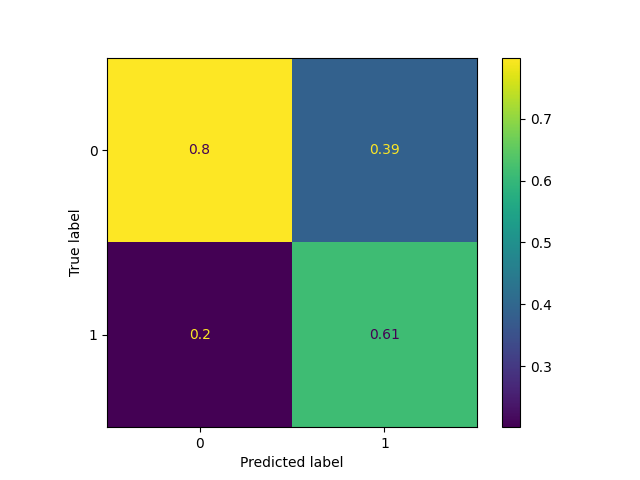
\includegraphics[width=13cm]{Results/Figures/confusion_matrix.png}
\end{figure}

\begin{figure}[H]
\caption{loss of fine tuning without reason}
\centering
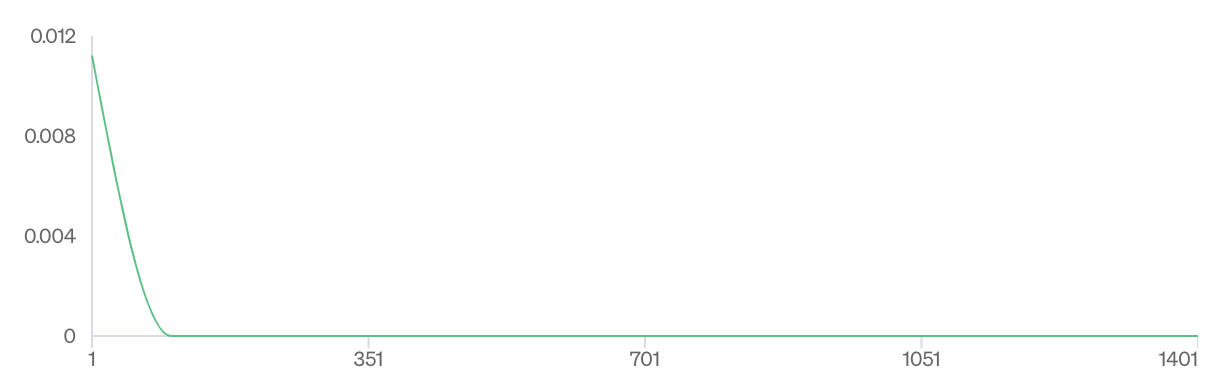
\includegraphics[width=17cm]{Results/Figures/no_reason_1000.png}
\end{figure}

\begin{figure}[H]
\caption{loss of fine tuning with reason}
\centering
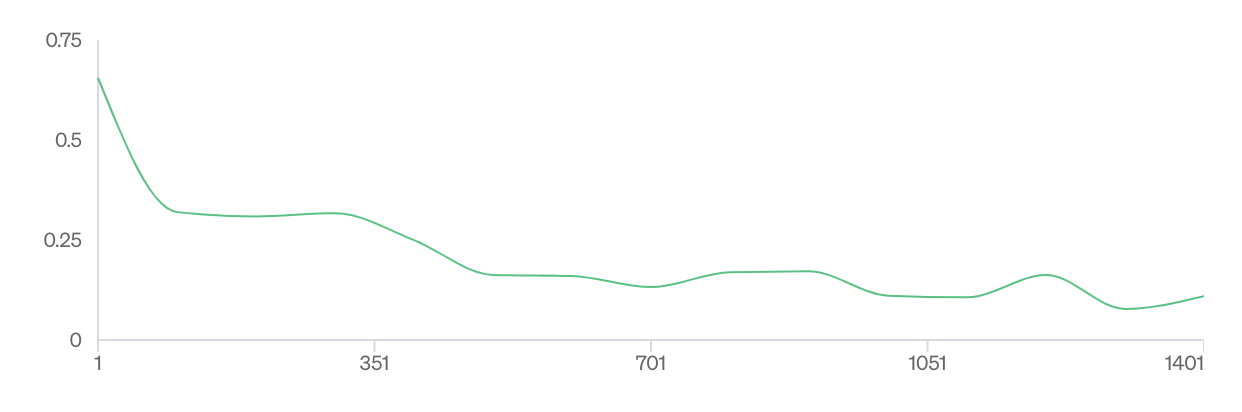
\includegraphics[width=17cm]{Results/Figures/with_reason_1000.png}
\end{figure}

\newpage



\begin{appendices}
\end{appendices}


\end{document}
